\documentclass[10pt,letterpaper]{article}
\RequirePackage{amsthm,amssymb,amsmath,graphicx}
\RequirePackage[top=2cm, bottom=2cm, left=2.5cm, right=3cm]{geometry}
\usepackage{caption}
\usepackage{subcaption}
\usepackage[pagebackref=false,colorlinks,linkcolor=black,citecolor=magenta]{hyperref}
\RequirePackage{MnSymbol}
\newcommand{\eqn}[2]{
\begin{equation}
\begin{split}
#1
\label{#2}
\end{split}
\end{equation}
}
%%%%%%%%%%%%%

%       \eqn{
%       x=x^2
%       }{label}

%%%%%%%%%%%%%
\newcommand{\feqn}[2]{
\begin{tcolorbox}[width=7in, colback=white]
\begin{equation}
\begin{split}
#1
\label{#2}
\end{split}
\end{equation}
\end{tcolorbox}
}
%%%%%%%%%%%%%%%
\newcommand{\hl}{
\begin{center}
\line(1,0){450}
\end{center}}
\setlength{\parindent}{0pt}
\newcommand{\nl}{\newline\newline}
\newcommand{\pic}[1]{
\begin{center}
\includegraphics[width=130mm]{#1}
\end{center}
}
%\settextfont{B Nazanin}
\usepackage{lipsum}
\begin{document}
\Large
\begin{center}
The assignment \#8 of the \textbf{ComNet} course
\hl
\end{center}
Q1) 

a) Why are multiple access protocols needed for transmission into a shared broadcast channel?

b) What does a node do when experiencing a collision in random access protocols? What is the benefit of this technique?
\newline
\newline
Q2)

Consider slotted ALOHA for multiple access transmission. Assume that each node, starts transmitting with probability $p$ at each time slot and there are $N$ nodes in total. Each frame exactly fits to each time slot (i.e. $F=R\times T$ where $F$, $R$ and $T$ are frame length, link capacity and time slot length, respectively). How many times (i.e. at how many time slots), in average, should a node send a frame in consecutive time slots to make sure the frame has been correctly received? Does the derived formula contain an optimum as a function of $p$? If so, find it and if not, explain why.
\newline
\newline
Q3)

Consider the previous question assuming that FDMA is utilized. Assume that the link capacity $R$ has been divided equally among $N=10$ users. Find the maximum available throughput for slotted ALOHA in the previous question by triggering $p$ and the effective throughput of FDMA for each user (we know that a user definitely transmits at each of its own time slots, ) and campare them. Does slotted ALOHA save bandwidth campared to FDMA? If so, how much?
\newline
\newline
Q4)

Consider the single switch VLAN in Figure 5.25, and assume an external
router is connected to switch port 1. Assign IP addresses to the EE and CS
hosts and router interface. Trace the steps taken at both the network layer and the link layer to transfer an IP datagram from an EE host to a CS host (Hint: reread the discussion of Figure 5.19 in the text).
\newline\newline
Q5)

In the following network, assume the red squares be layer-2 switches and the green circles as hosts (the tiny numbers denote the interface IDs. Also the switches S1 and S4 are connected through a wireless connection):
\begin{center}
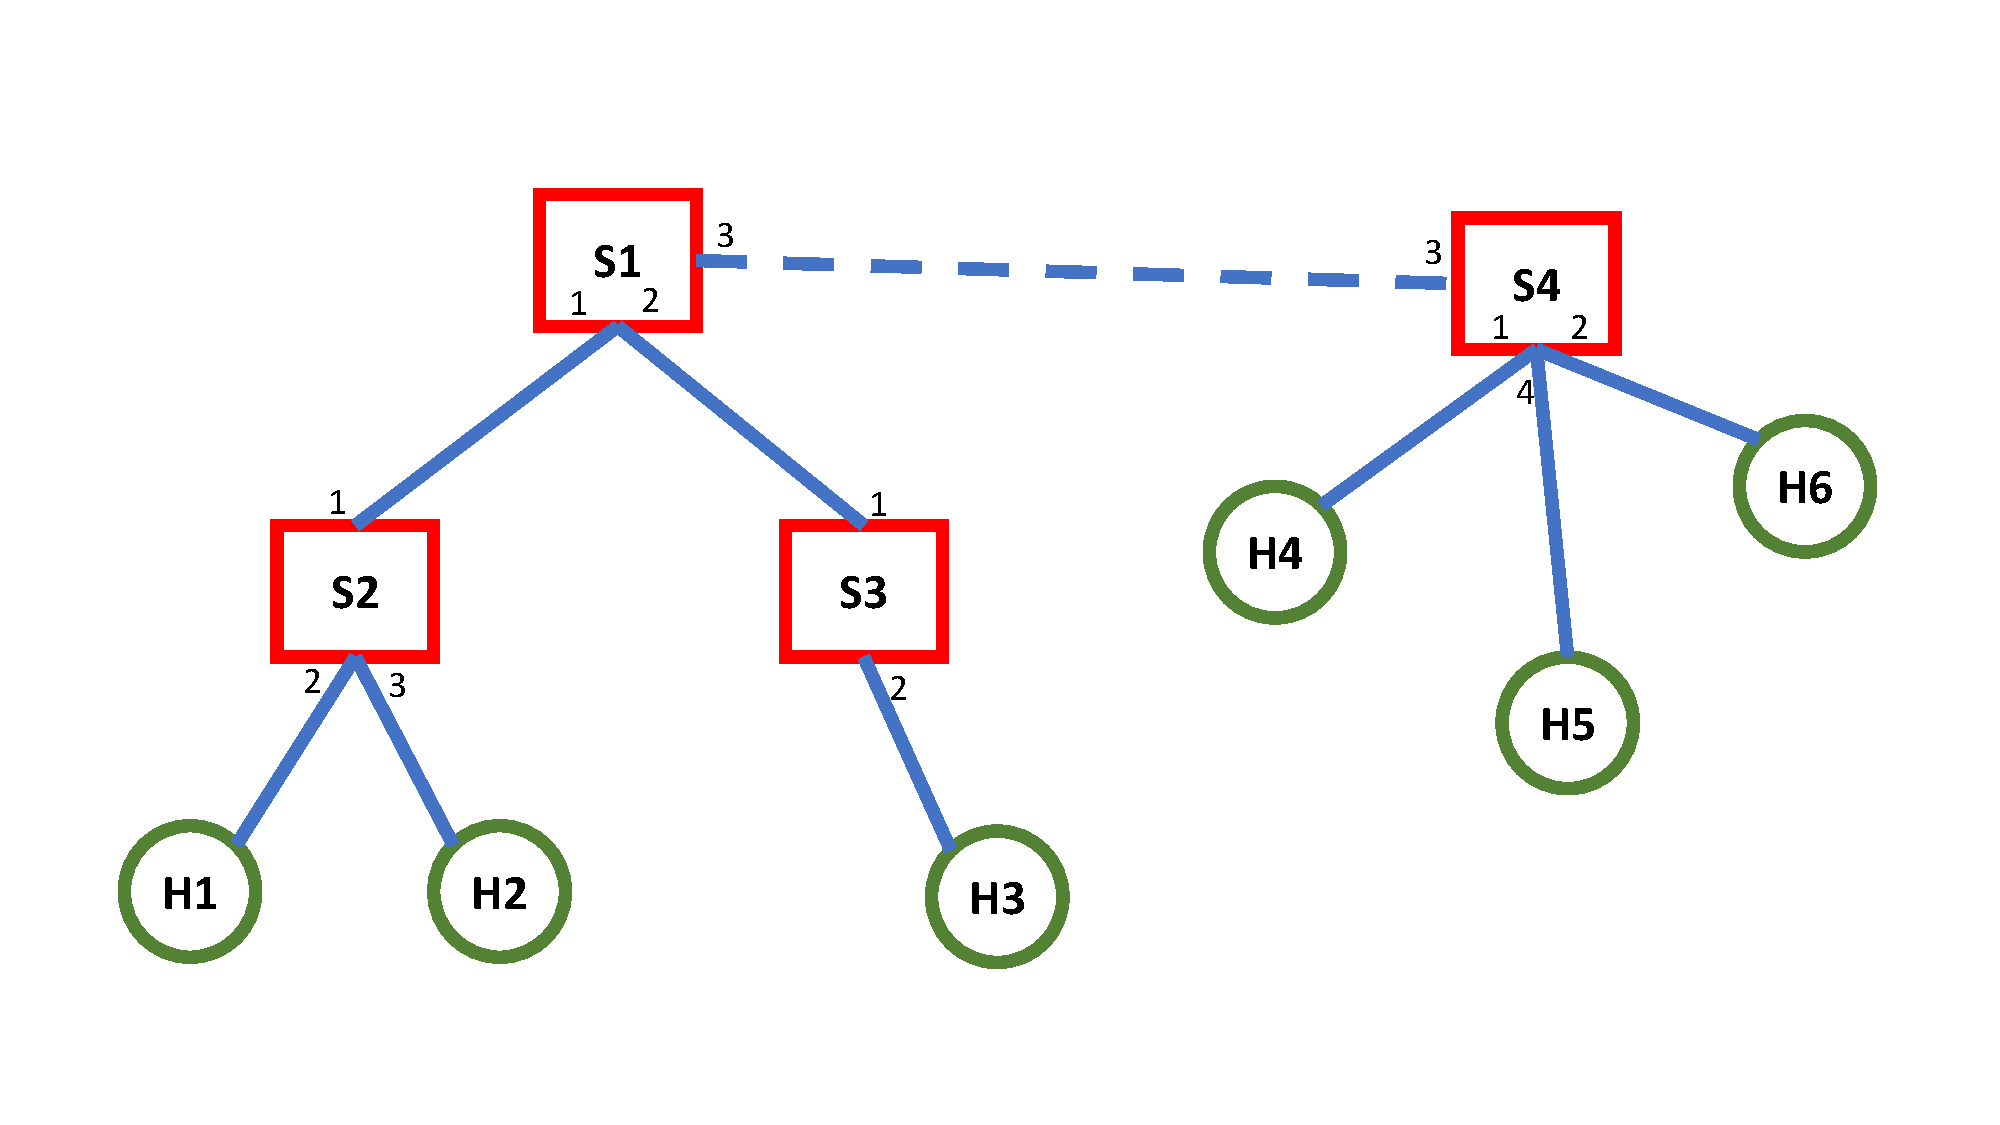
\includegraphics[width=120mm]{Q5_HW8}
\end{center}
a) What information is stored in all the switches when the host H1 with MAC address AA:AA:AA:AA:AA:AA broadcasts a frame considering the self-learning phase? (Drop the TTL arbitrarily in this part)

b) Assume that the host H3 wants to send a packet to H6 while the information of H6 are not recorded in S4 switch table. Where does the switch S4 forward the upstream packet?
\newline\newline
Q6)

Remember the discussion about Ethernet frames and the preamble header field. As explained before, an Ethernet frame starts with 8 bytes of preamble. Each of the first 7 bytes are $10101010$ while the last one is $10101011$. Assume that once the receiver grabs a byte $10101011$ from the channel, it considers that the rest of the Ethernet frame is about to come and the next incoming bytes are the main data. If at least one of the first 8 bytes of the Ethernet frame is not either $10101010$ or $10101011$, the frame is dropped. The channel reverts each bit with a probability of $p$.

a) What is the probability that an error occurs in the preamble and the receiver does not correctly detect the rest of the Ethernet frame assuming that the sender has sent a group of 7 bytes of $10101010$ followed by $10101011$ as preamble?

b) Suppose that only the preamble field is error-prone (the rest of Ethernet frame remain still). How much decrease in probability of error in part ``a'' is obtained if we use the parity-check method with a single parity bit instead of CRC? (The Ethernet frames with incorrect digit sum are dropped)
\end{document}